\chapter{PTAS for Graphs of Bounded Genus}
\label{chapter:ptas_bounded_genus}

\section{Algorithm Overview}

As we shall see, the proposed PTAS for \steinercycle\ is inspired by the PTAS for the Steiner Tree Problem due to \cite{Bateni}. Put briefly, the proposed algorithm for \steinercycle\ consists of the following steps:

\begin{enumerate}
    \item The algorithm receives as input a graph \(G_{in}\) with bounded genus, and a set \(\mathcal{D} = \{T_1, \dots, T_k\}\) of terminal pairs.

    \item It begins by creating a spanner subgraph (i.e., a subgraph whose size is bounded by a constant time \(\opt\) and has a valid solution with a cost at most \((1 + \epsilon) \opt\) of \(G_{in}\). This is done with an auxiliary clustering algorithm provided by Theorem~\ref{theoremClustering}.

    \item The edges of the spanner are split into \(k\)-disjoint sets, then the edges in the smallest set are contracted. After the contraction, the algorithm applies \citeauthor{Demaine2010}'s Theorem (\cite{Demaine2010} Theorem~1.1) to convert the spanner subgraph to a bounded treewidth graph.

    \item The algorithm then applies the PTAS for bounded treewidth graphs, which is presented in Chapter~\ref{chapter:ptas_bounded_tree}. This step returns a solution with cost of at most a costant times \(\opt\).

    \item Finally, it constructs the final solution, i.e., the PTAS for bounded genus, by leveraging the solution in bounded treewidth and the set of edges contracted in the previous step.
\end{enumerate}

\section{Prize Collecting Partition}
\label{section:pc-partition}

In this section we start presenting some necessary tooling for the construction of the PTAS for SMCP on bounded treewidth graphs and, subsequently, on bounded genus graphs. You can see an overview of the 

This section aims to prove the Prize Collecting Partition Theorem (Theorem~\ref{theoremClustering}) presented below, allowing us to break a Steiner Multicycle instance into simpler, smaller ones. The proof relies upon an algorithm called Prize-Collecting Clustering, or PC-clustering, which will be presented later in this section.

\begin{ftheo}~\label{theoremClustering}
Given an \(\epsilon > 0\), a graph \(G_{in}\), a cost function associated with each edge in \(E(G_{in})\), and a set \(\mathcal{D}\) of terminal pairs, we can compute in polynomial time a set of disjoint components \(\{C_1, \dots, C_k\}\) (i.e., a set of subgraphs of \(G_{in}\)) with an associated partition of the set of terminal pairs \(\{\mathcal{D}_1, \dots, \mathcal{D}_k\}\) with the following properties:
\begin{enumerate}
    \item All sets of terminal pairs are covered, that is, \(\mathcal{D} = \bigcup_{i=1}^k \mathcal{D}_i\); \label{condition_t_clust:1}
    \item All the terminals pairs in \(\mathcal{D}_i\) are covered by the component \(C_i\); \label{condition_t_clust:2}
    \item The sum of the cost of all the components \(C_i\) is no more than \((16/\epsilon + 4) \opt_{\mathcal{D}}(G_{in})\); \label{condition_t_clust:3}
    \item The sum of the costs of the minimum collection of cycles for each set of terminal pairs \(\mathcal{D}_i\) is no more than \(1 + \epsilon\) times the cost of a minimum solution of the SMCP in \(G_{in}\); that is, \(\sum_i \opt_{\mathcal{D}_i} (G_{in}) \leq (1 + \epsilon) \opt_{\mathcal{D}} (G_{in})\). \label{condition_t_clust:4}
\end{enumerate}
\end{ftheo}

The last condition implies that we can solve the problem in each \(C_i\) separately and still guarantee an approximation with a small factor.

We start proving Theorem~\ref{theoremClustering} by applying a 4-approximation algorithm in \(G_{in}\) (for instance, the algorithm for SMCP provided by \cite{Pereira2018TheSM}). Clearly, this construction satisfies the first two properties, since by definition an SMCP solution covers all sets, and for each set \(\mathcal{D}_i\) a component in the solution connects all of its terminal pairs. To guarantee the last two properties, we need to employ the \textbf{PC-clustering} algorithm, which is presented in Section~\ref{subsection:pc_clustering}.

\subsection{Prize-Collecting Clustering}~\label{subsection:pc_clustering}

The PC-Clustering algorithm is used in the proof of the following theorem - which in turn will be used to prove Theorem~\ref{theoremClustering}. 
It is worth mentioning that the Theorem~\ref{theoremClustering_Bateni_3_1} is based on \cite{Bateni} (see Theorem 3.1 (Prize-Collecting Clustering)).

\begin{ftheo} \label{theoremClustering_Bateni_3_1}
Let \(G=(V, E)\) be a graph with a nonnegative edge cost \(c(e)\) for each edge \(e\) and a potential \(\phi_v\) for each vertex \(v \in V\). 
There is a polynomial-time algorithm that computes a subgraph \(Z\) of \(G\) such that:

\begin{enumerate}
    \item the cost of \(Z\) is at most \(4 \sum \limits_{v \in V} \phi_v\), and~\label{condition:1}
    \item \(Z\) is a spanning subgraph of \(G\), and~\label{condition:2}
    \item all vertices in \(Z\) have even degree, and~\label{condition:3}
    \item for any subgraph \(L\) of \(G\), there is a set  of vertices \(Q\) such that: \label{condition:4}
    \begin{enumerate}
        \item \(\sum \limits_{v \in Q} \phi_v\) is at most the cost of \(L\), and \label{condition:4a}
        \item if two vertices \(v_1, v_2 \notin Q\) are connected by \(L\), then they are  in the same component of \(Z\).~\label{condition:4b}
    \end{enumerate}
\end{enumerate}
\end{ftheo}

The statement above might look too abstract at first, but it will get more clear with its proof and application. First let us present a brief overview of the PC-Clustering algorithm, followed by a more complete description.

We start with a graph where vertices have associated potentials (or prizes) and edges have a ``crossing cost''. The idea is to agglomerate the vertices into disjoint clusters progressively. 

Initially, each vertex induces an individual cluster. The total potential of a cluster equals the sum of the potentials of its internal vertices minus the cost of its internal edges. At each step, clusters can use their potential to ``pay'' for crossing edges to merge with other clusters. That way, the algorithm iteratively spends the potential of the graph's vertices until all the potential is spent.

\cite{Bateni} make an analogy to edge painting while presenting the algorithm, where each vertex is associated with a color, and its colors are used to paint edges to connect separated clusters; when an edge is fully painted, it merges two clusters.

To summarize, at the beginning of the algorithm, each vertex \(v\) of \(V(G)\) has a potential \(\phi_v\) that can be spent in clusters that contain \(v\) (so this cluster can connect to other clusters to form new bigger clusters). We keep track of how much ``potential'' the vertex \(v\) spent on a cluster \(S\) via the variable \(\gamma_{S, v}\), where \(S \subseteq V(G): v \in S\). Given a cluster \(C\), we generalize the variable \(\gamma\) as \(\gamma_{C}:= \sum_{v \in C} \gamma_{C, v}\) to account for the total potential spent by any vertex in the cluster \(C\).

The algorithm consists of two stages: \textit{growth} and \textit{pruning}. At the growth stage, we aim to find a subgraph \(F_1\) and a corresponding \(\gamma\). Next, we \textit{prune} (i.e., remove) some of the edges of \(F_1\) to get another subgraph \(F_2\). Finally, we duplicate all edges in \(F_2\) to obtain \(M_2\).

Noticeably, the following inequalities must be respected throughout the whole process.

\begin{align}
&&\sum_{S\subseteq V(G): e \in \delta(S)} \sum_{v \in S} \gamma_{S, v} \leq c(e) && \forall e \in E(G) \label{ineq:1} \\
&&\sum_{S \subseteq V(G): S \ni v} \gamma_{S, v} \leq \phi_v && \forall v \in V \label{ineq:2} \\
&&\gamma_{S, v} \geq 0 && \forall S \subseteq V(G), v \in S \label{ineq:3}
\end{align}

The main goal of the growth stage is to build a spanning subgraph \(F_1\) that partitions the vertices of \(G\). The intuition is to think of \(\phi_v\) as an amount of potential that \(v\) can spend in a cluster \(S\), to which it belongs (i.e., \(v \in S\)), to merge \(S\) with other clusters in \(G\). However, that must be done in a way that the total spent to cross an edge is no more than the cost of that edge (Constraint~\eqref{ineq:1}), and that vertex \(v\) of \(S\) does not use more potential than it has available (Constraint~\eqref{ineq:2}). The Constraint~\eqref{ineq:3} ensures that the value that \(v\) contributes to \(S\) is never negative.

We begin the growth stage with an empty \(\gamma\) (i.e., \(\forall v \in V(G)\) and \(\forall S \subseteq V(G)\) we have \(\gamma_{v, S} = 0\)) and a subgraph \(F_1\) also empty (i.e., has no edges). During this step, we keep track of a set of clusters \(\mathcal{C}\) which partitions the vertices of \(V(G)\); initially, each cluster is composed of a single vertex. We say that a cluster \(C \in \mathcal{C}\) is \textbf{active} if \(\sum_{C' \subseteq C} \sum_{v \in C'} \gamma_{C', v} < \sum_{v \in C} \phi_v\) (i.e. the cluster \(C\) still has vertices with remaining potential). Notice that if a vertex \(v \in C_1 \subset C_2\) spent \(\gamma_{C_1, v}\) to join \(C_1\) with another cluster to form \(C_2\), the potential \(\gamma_{C_1, v}\) cannot be used in \(C_2\). We say that a vertex is active if it still has some spending potential.

During the growth process, we iteratively spend potential from vertices to grow all active clusters by a value \(\eta\) - which may vary between iterations. It is important to note that an equal amount of \(\eta\) is spent on each cluster within the same iteration, and for each cluster, each of its active vertices spends the same amount of potential. Thus, it is possible for the amount spent between vertices of different clusters to be different, depending on the number of active vertices in each cluster.

Let us consider a specific cluster \(C\) and denote by \(\kappa(C)\) as the number of active vertices in \(C\). Each active vertex in \(C\) spends \(\eta / \kappa(C)\) of its available potential into the cluster \(C\). This implies that a total of \(\eta\) will be spent on \(C\) during the iteration.
The value of \(\eta\) is the largest possible value that still adheres to the Constraints~\eqref{ineq:1},~\eqref{ineq:2} and~\eqref{ineq:3} for all active clusters.

After each growth iteration, some constraints might reach equality. If Constraint~\eqref{ineq:2} becomes tight for some vertices, then those vertices become inactive. 
If all vertices inside a cluster become inactive, then we say that the cluster itself becomes inactive. 
In case Constraint~\eqref{ineq:1} becomes tight for some edge \(uv\), then the potential spent by two neighboring clusters was enough to cover the cost of the edge. This implies that there are two clusters \(C_u \ni u\) and \(C_v \ni v\) which we can merge into a new cluster \(C = C_u \cup C_v\), by adding \(uv\) to \(F_1\). We then add the new cluster and remove the two former clusters from \(\mathcal{C}\).

Note that after each growth iteration, at least one of the restrictions will meet equality for some set of vertices and/or edges. Thus, after a polynomial number of iterations, either all restrictions are met in equality, or the potential of all vertices is spent.

The pruning stage iteratively removes some edges from \(F_1\) to form \(F_2\). This process is necessary for proving Lemma~\ref{clustering_connecting_bateni_3_4}. Let \(\mathcal{S}\) be the set containing all sets that were a cluster at some point during the growth stage. It can be easily observed that the clusters in \(\mathcal{S}\) are laminar and the maximal clusters are the clusters of \(\mathcal{C}\). Note that \(F_1[C]\) is connected for each \(C \in \mathcal{S}\).

Let \(\mathcal{B} \subseteq \mathcal{S}\) be the set of all tight clusters at the end of the growth stage, i.e., for each \(S \in \mathcal{B}\) we have \(\sum_{S' \subseteq S} \sum_{v \in S'} \gamma_{S', v} = \sum_{v \in S} \phi_v\). At the beginning of the stage, we initialize \(F_2\) as \(F_1\). While there is a cluster \(S \in \mathcal{B}\) such that \(F_2 \cap \delta(S) = \{e\}\) (notice that if \(F_2 \cap \delta(S)\) has more than one edge we do not prune \(S\)), we remove the edge \(e\) from \(F_2\).

At the end of this process, \(F_2\) does not have edges of \(\delta(C)\), for each \(C \in \mathcal{S}\); in other words, no connected component of \(F_2\) can have two vertices such that one belongs to \(C\) and the other does not. Finally, we duplicate the edges of \(F_2\) to form \(M_2\).

For Algorithm~\ref{algorithm:pc-clustering}, we define \(\mathcal{C}(v)\) as the cluster currently containing the vertex \(v \in V\), that is, \(\mathcal{C}(v):= C\) for any \(v \in C \in \mathcal{C}\).

\begin{algorithm}[H]
\caption{PC-Clustering}
\label{algorithm:pc-clustering}
\begin{algorithmic}[1]

\Require Graph \(G\), and potentials \(\phi_v > 0\).
\Ensure Subgraph \(M_2\).

\State Let \(F_1 \gets (V(G), \emptyset)\).
\State Let \(\gamma_{S, v} \gets 0\) for any \(S \subseteq V : v \in S\).
\State Let \(\mathcal{S} \gets \mathcal{C} \gets \{\{v\}: v \in V(G)\}\).
\While {there is an active vertex} \label{alg:line-while}
    \State Let \(\eta\) be the largest possible value such that simultaneously increasing \(\gamma_C\) by \(\eta\) for all active clusters \(C\) does not violate Constraints \eqref{ineq:1}, \eqref{ineq:2} and \eqref{ineq:3}.
    \State Let \(\gamma_{\mathcal{C}(v), v} \gets \gamma_{\mathcal{C}(v), v} + \frac{\eta}{\kappa(\mathcal{C}(v))}\) for all active vertices \(v\).
    \If {\(\exists e \in E(G)\) that is tight and connects two clusters}
        \State Pick one such edge \(e = \{u, v\}\).
        \State Let \(F_1 \gets F_1 \cup \{e\}\).
        \State Let \(C \gets \mathcal{C}(u) \cup \mathcal{C}(v)\).
        \State Let \(\mathcal{C} \gets \mathcal{C} \cup \{C\} \backslash \{ \mathcal{C}(u), \mathcal{C}(v) \}\).
        \State Let \(\mathcal{S} \gets \mathcal{S} \cup \{C\}\).
    \EndIf
\EndWhile

\State Let \(F_2 \gets F_1\).
\State Let \(\mathcal{B} \gets \{S \in \mathcal{S} : \sum_{S' \subseteq S} \sum_{v \in S'} \gamma_{S', v} = \sum_{v \in S} \phi_v\}\).
\While {\(\exists S \in \mathcal{B}\) such that \(F_2 \cap \delta(S) = \{e\}\) for an edge \(e\)}
    \State Let \(F_2 \gets F_2 \backslash \{e\}\).
\EndWhile
\State Duplicate edges of \(F_2\) to form \(M_2\).
\State Output \(M_2\).

\end{algorithmic}
\end{algorithm}

\begin{flemma}[\cite{Bateni} - Lemma 3.3] \label{clustering_bound_bateni_3_3}
    The cost of \(F_2\) is at most \(2 \sum_{v \in V} \phi_v\).
\end{flemma}
\begin{proof}
The PC-Clustering algorithm has a notion of time. At each discrete step of the algorithm (i.e., at each iteration of line~\ref{alg:line-while}), one of two events happens: a cluster becomes inactive, or an edge becomes tight. We call the ``time'' between two event points \textbf{epoch}. 

Notice that, during each epoch, each cluster is either active or inactive, and each active cluster \(C\) increases its \(\gamma_C\) value, while all other \(\gamma\)'s remain unchanged. At time \(0\), all (singleton) clusters with a strictly positive penalty are active.

We aim at proving that the cost of \(F_2\) is at most \(2 \sum_{S \subseteq V : v \in S} \gamma_{S, v} \leq 2 \sum_{v \in V} \phi_v\), where the inequality follows from Constraint~\eqref{ineq:2}.

Let \(t_j\) be the time at which the \(j^{th}\) event point occurs in the growth step. So the \(j^{th}\) epoch is the time interval between \(t_{j-1}\) to \(t_j\). For each cluster \(C\) let \(\gamma_{C}^{(j)}\) be the amount \(\gamma_{C}:= \sum_{v \in C} \gamma_{C, v}\) that the cluster grew during epoch \(j\), which is  \(t_j - t_{j-1}\) if it was active during this epoch, or zero otherwise. Thus, \(\gamma_C = \sum_j \gamma_C^{(j)}\).

Since each edge \(e\) of \(F_2\) was added at some point by the growth stage when its edge packing Constraint~\eqref{ineq:1} became tight, we can exactly apportion the cost \(c(e)\) amongst the collection of clusters \(\{K: e \in \delta(K)\}\) whose variables ``paid for'' the edge, and can divide this up further by epoch. In other words, \(c(e) = \sum_j \sum_{K : e \in \delta (K)} \gamma_K^{(j)}\). Summing over the epochs yields the desired conclusion.

We will now prove that, for an arbitrary epoch \(j\), the total edge cost of \(F_2\) that is apportioned from epoch \(j\) is at most \(2 \sum_C \gamma_C^{(j)}\). In other words, the total rate at which all active clusters pay for edges of \(F_2\) is at most twice the available potential of the active clusters during the epoch.

Let \(\mathcal{C}_j\) be the set of clusters that existed during epoch \(j\) (either active or inactive). Consider the graph \(F_2\) and then collapse each cluster \(C \in \mathcal{C}_j\) into a supernode. Let \(H\) be the resulting graph. We will continue to refer to each supernode as a ``cluster'' during the rest of the proof. Let us denote the active and inactive clusters in \(\mathcal{C}_j\) by \(\mathcal{C}_{act}\) and \(\mathcal{C}_{dead}\), respectively.

The edges of \(F_2\) that are being partially paid during epoch \(j\) are exactly those edges of \(H\) that are incident to an active cluster -- and the total amount of these edges that are being paid during epoch \(j\) is \((t_j - t_{j - 1}) \sum_{C \in \mathcal{C}_{act}} deg_H(C)\). Since every active cluster grows by exactly \(t_j - t_{j - 1}\) in epoch \(j\), we have:

$$\sum_C \gamma_C^{(j)} \geq \sum_{C \in \mathcal{C}_j} \gamma_C^{(j)} = (t_j - t_{j - 1}) |\mathcal{C}_{act}|$$

Now we show that \(\sum_{C \in \mathcal{C}_{act}} deg_H(C) \leq 2|\mathcal{C}_{act}|\).

Since each cluster induces a connected subtree of \(F_1\) and \(H\) is built from the contraction of edges of \(F_2\), it does not introduce new cycles, which implies that \(H\) is a forest. 
Also, all the leaves in \(H\) must be active, because otherwise the corresponding cluster would have been pruned into another component during the pruning stage.

With this information about \(H\), it is easy to bound \(\sum_{C \in \mathcal{C}_{act}} deg_H(C)\). The total degree in \(H\) is at most \(2 (|\mathcal{C}_{act}| + |\mathcal{C}_{dead}|)\). Noticing that the degree of dead clusters is at least two, we get \(\sum_{C \in \mathcal{C}_{act}} deg_H(C) \leq 2 (|\mathcal{C}_{act}| + |\mathcal{C}_{dead}|) - 2|\mathcal{C}_{dead}| = 2|\mathcal{C}_{act}|\) as desired.

Finally, we obtain the following inequality because $t_j-t_{j-1} \ge 0$:

$$(t_j - t_{j - 1}) \sum_{C \in \mathcal{C}_{act}} \mathrm{deg}_H(C) \leq 2 (t_j - t_{j - 1}) |\mathcal{C}_{act}|$$

Since the left-hand side of the inequality is the total amount being paid to edges of \(F_2\) during epoch \(j\), by summing through all epochs, we get:

$$c(F_2) \leq 2 \sum_j \sum_C \gamma_C^{(j)} = 2 \sum_{S \subseteq V : v \in S} \gamma_{S, v} \leq 2 \sum_{v \in V} \phi_v.$$

\end{proof}

Let \(M_2\) be the graph created by duplicating each edge on \(F_2\). Notice that all vertices in \(M_2\) have even degrees and, besides that, \(c(M_2) \leq 4 \sum_{v \in V} \phi_v\), which is formalized in the following result.

\begin{fcorollary}~\label{corollary_1}
The cost of the graph \(M_2\) is at most \(4 \sum_{v \in V} \phi_v\).
\end{fcorollary}
\begin{proof}
    The result follows immediately from Lemma~\ref{clustering_bound_bateni_3_3}.
\end{proof}

The following lemma due to~\cite{Bateni} gives a sufficient condition for two vertices that end up in the same component of \(F_2\).

\begin{flemma}[\cite{Bateni} - Lemma 3.4] \label{clustering_connecting_bateni_3_4}
    Two vertices \(u\) and \(v\) of \(V(G)\) are connected in \(F_2\) if there exist clusters \(S, S'\) both containing \(u\) and \(v\) such that \(\gamma_{S, v} > 0\) and \(\gamma_{S', u} > 0\).
\end{flemma}
\begin{proof}

    The growth stage connects \(u\) and \(v\) since \(\gamma_{S, v} > 0\) and \(u, v \in S\). Consider the path \(P\) connecting \(u\) and \(v\) in \(F_1\). All the vertices of \(P\) are in \(S\) and \(S'\). For the sake of reaching a contradiction, suppose some edges of \(P\) are pruned. Let \(e\) be the first edge being pruned in \(P\). 

    Thus, there must be a cluster \(C \in \mathcal{B}\) which cuts \(e\) (i.e. \(C\) only contains one endpoint of the edge \(e\)); furthermore, \(\delta(C) \cap E(P) = \{e\}\), since \(e\) is the first edge pruned from \(P\). As \(C\) cuts \(e\), the laminarity of the clusters gives \(C \subset S, S'\).

    In addition, note that \(C\) contains precisely one endpoint of the path \(P\) (as opposed to precisely one endpoint of the edge \(e\)). This holds because if \(C\) contained neither or both endpoints of \(P\), so the cluster \(C\) could not cut \(P\) at exactly one edge.

    Let \(v\) the endpoint of \(P\) in this cluster. We then have \(\sum_{C' \subseteq C} \gamma_{C',v} = \phi_v\) because \(C\) is tight. However, as \(C\) is a \textit{proper} subset of \(S\), this contradicts with \(\gamma_{S, v} > 0\), proving that the supposition is false. The case when \(C\) contains \(u\) is symmetric.
\end{proof}

As mentioned before, \citeauthor{Bateni} associate a color to each vertex so that the vertex ``spends'' its color to fill the edges. Therefore, we say that a cluster \(H\) exhausts a vertex's \(v\) color, when \(\sum_{C \subseteq H} \gamma_{C, v} = \phi_v\). This analogy will be mentioned in the lemmas ahead.

\begin{flemma}[\cite{Bateni} Lemma 3.5]~\label{clustering_bateni_3_5}
    If a subgraph \(H\) of \(G\) connects two vertices \(u, v\) from different components of \(F_2\), then \(H\) exhausts the ``color'' corresponding to at least one of \(u\) and \(v\).
\end{flemma}
\begin{proof}
    Given that \(H\) connects \(u\) and \(v\), suppose that \(H\) exhausts neither \(u\) nor \(v\): there is a set \(S\) containing \(u\) and a set \(S'\) containing \(v\) such that \(\gamma_{S, v} > 0\) and \(\gamma_{S', u} > 0\) and \(E(H) \cap \delta(S) = E(H) \cap \delta(S') = \emptyset\). Since \(H\) connects \(u\) and \(v\), this is only possible if \(u\) and \(v\) are both in \(S\) and \(S'\). By Lemma~\ref{clustering_connecting_bateni_3_4}, this implies that \(F_2\) connects \(u\) and \(v\), a contradiction.
\end{proof}

We can relate the cost of a subgraph to the potential value of the colors it exhausts.

\begin{flemma}[\cite{Bateni} Lemma 3.6] \label{clustering_bateni_3_6}
    Let \(Q\) be the set of colors exhausted by subgraph \(G'\) of \(G\). The cost of \(G'\) is at least \(\sum_{v \in Q} \phi_v\).
\end{flemma}
\begin{proof}
    This is quite intuitive. Recall that vertices have associated ``colors'' which are used to ``color'' the edges of \(G\) during cluster growth. Consider a segment on edges corresponding to cluster \(S\) with color \(v\). At least one edge of \(G'\) passes through the cut \((S, \overline{S})\). Thus, a portion of the cost of \(G'\) can be charged from \(\gamma_{S, v}\). Hence, the total cost of the graph \(G'\) is at least as large as the total amount of colors paid for by \(Q\).
\end{proof}

We  finally have all tools to prove Theorem~\ref{theoremClustering_Bateni_3_1}.

\begin{proof}[Proof of Theorem~\ref{theoremClustering_Bateni_3_1}]
The subgraph \(Z\) is the graph \(M_2\), which corresponds to the forest \(F_2\) with duplicated edges, which already guarantees Condition~\eqref{condition:3}.

Condition~\eqref{condition:1} is given by Corollary~\ref{corollary_1}. 

To assert Condition~\eqref{condition:2}, we must observe that, as a first step of the growth stage of the Algorithm~\ref{algorithm:pc-clustering}, we initialize each vertex as an individual cluster.

For Condition~\eqref{condition:4}, let \(Q\) be the set of vertices exhausted by \(L\). Conditions~\eqref{condition:4a} and~\eqref{condition:4b} are proved by Lemma~\ref{clustering_bateni_3_6} and Lemma~\ref{clustering_bateni_3_5}, respectively.

\end{proof}

\subsection{Proof of PC-Partition Theorem}

The proof of the PC-Partition Theorem (Theorem~\ref{theoremClustering}) induces an algorithm that outputs a set of components of an input graph \(G_{in}\). Such an algorithm is presented in Algorithm~\ref{algorithm:pc-partition}.

\begin{algorithm}[H]
\caption{PC-Partition}
\label{algorithm:pc-partition}
\begin{algorithmic}[1]

\Require Graph \(G_{in}\), a set of costs associated with the edges in \(E{G_{in}}\) and a set of terminal pairs \(\mathcal{D}\)
\Ensure Set of components \(\{C_i\}_{i=1}^k\) such that \(C_i\) covers the terminals in \(\mathcal{D}_i\)
\State Use the algorithm proposed by \cite{Pereira2018TheSM} to find a Steiner Multicycle 4-approximated \(M^\ast = \{C^\ast_1, \dots, C^\ast_k\}\) of \(\mathcal{D}\).
\State Contract each cycle \(C_i^\ast\) in order to create a new graph \(G\).
\State For every \(v \in V(G)\), let \(\phi_v\) be equal to \(\frac{1}{\epsilon}\) times the cost of the cycle \(C_i^\ast\) that was contracted into \(v\), and \(0\) in case there is no such cycle.
\State Let \(M_2\) be the solution produced by the PC-Clustering algorithm on \(G\) and \(\phi_v\).
\State Build \(M\) from \(M_2\) by \emph{uncontracting} all cycles \(C_i^\ast\).
\State Return the set of components \(\{C_i\}_{i=1}^k\), with \(\mathcal{D}_i := \{(s, t) \in \mathcal{D}: s, t \in V(C_i)\}\).

\end{algorithmic}
\end{algorithm}

\begin{proof}[Proof of Theorem~\ref{theoremClustering}]

Let \(G\) be the graph resulting from the contraction of the components of the 4-approximation \(M^\ast\) (as shown in Algorithm~\ref{algorithm:pc-partition}). For each component \(C\) of \(M^\ast\) contracted, resulting in a vertex \(v\), we define a potential \(\phi_v := \frac{1}{\epsilon} \cdot c(C)\) if \(v\) is the result of the contraction of a component of \(M^\ast\) and zero otherwise. 

Let \(Z\) be the subgraph of \(G\) given by Theorem~\ref{theoremClustering_Bateni_3_1}. Let \(Z_{in}\) be the subgraph of \(G_{in}\) obtained from \(Z\) by uncontracting the components of \(M^\ast\) and adding \(M^\ast\) to \(Z_{in}\). Note that \(Z_{in}\) is a spanning subgraph of \(G_{in}\), since \(Z\) is a spanning subgraph of \(G\) (Condition~\eqref{condition:2}).

Considering that \(M^\ast\) is a valid solution, and each vertex in \(Z\) has an even degree (Condition~\eqref{condition:3}), we have that \(Z_{in}\) is a valid solution for the SMCP as well. Let \(\{C_1, \dots, C_k\}\) be the components of \(Z_{in}\), and let \(\mathcal{D}_1, \dots, \mathcal{D}_k\) be the set of terminal pairs covered by those components. It is clear that \(Z_{in}\) satisfies Conditions~\eqref{condition_t_clust:1} and~\eqref{condition_t_clust:2}.

To prove that \(Z_{in}\) satisfies Condition~\eqref{condition_t_clust:3}, note that the cost of \(Z_{in}\) is the cost of \(M^\ast\) (which is at most \(4 \cdot \opt\)) plus the cost of \(Z\) (which, by Theorem~\ref{theoremClustering_Bateni_3_1}, is at most \( 4 \sum_{v \in V} \phi_v = \frac{4}{\epsilon} c(M^\ast) \leq \frac{16}{\epsilon} \opt \) by construction).


\begin{figure}[H]
    \centering
% \tikzset{
%     every node/.style={
%         circle,
%         draw,
%         solid,
%         fill=black!50,
%         inner sep=0pt,
%         minimum width=4pt
%     }
% }
\begin{tikzpicture}[thick,scale=1.8,-,shorten >=2pt]

    \draw (0,0) node {} -- (1,1) [dashed] node {};
    \draw (2, 1.5) node {} -- (3,2) [dashed] node {};
    
    \draw (1,2) node {} -- (2, 1.5) [dashed] node {};

    \draw (3, 0.3) node {} -- (4,0) [dashed] node {};
    \draw (3, 0.3) node {} -- (4,-1) [dashed] node {};
    \draw (0,2) node {} -- (1,2) [dashed] node {};
    \draw (4,1) node {} -- (3, 0.3) [dashed] node {};


    \draw (1,1) node {} -- (2, 1.5) [red] node {};
    \draw (3.03,2) node {} -- (4.03,1) [red] node {};
    \draw (2.03, 1.5) node {} -- (2.03,0) [red] node {};   
    \draw (1,1.04) node {} -- (1,-0.26) [red] node {};
    \draw (1,-0.27) node {} -- (2,0.03) [red] node {};
    \draw (0.05,0) node {} -- (0.05,2) [red] node {};
    \draw (4.03,1) node {} -- (4.03,0) [red] node {};

    \draw  (0,2) node {} -- (1,1) [green] node {};
    \draw (0,0) node {} -- (1,-0.3) [green] node {};
    \draw (1,0.95) node {} -- (2, 1.45) [green] node {};
    \draw (2.97,2) node {} -- (3.98,1) [green] node {};
    \draw (1.97, 1.5) node {} -- (1.97,0) [green] node {};
    \draw (1,-0.33) node {} -- (2,-0.03) [green] node {};
    \draw (0,0) node {} -- (0,2) [green] node {};
    \draw (3.97,1) node {} -- (3.97,0) [green] node {};

    \Vertex[x=1, y=2, color=white]{A}
    \Vertex[x=4, y=1, color=white]{B}
    \Vertex[x=3, y=0.3, color=white]{C}
    \Vertex[x=4, y=-1, color=white]{D}

    \Vertex[x=0, y=2, label=$t_1$, color=white]{t_1}
    \Vertex[label=$t'_1$, color=white]{t_1'}

    \Vertex[x=1, y=1, label=$t_2$, color=white]{t_2}
    \Vertex[x=2, y=0, label=$t'_2$, color=white]{t_2'}

    \Vertex[x=1, y=-0.3, label=$t_3$, color=white]{t_3}
    \Vertex[x=2, y=1.5, label=$t'_3$, color=white]{t_3'}

    \Vertex[x=3, y=2, label=$t_4$, color=white]{t_4}
    \Vertex[x=4, y=0, label=$t'_4$, color=white]{t_4'}

\end{tikzpicture}

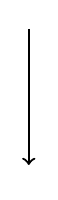
\begin{tikzpicture}[thick,scale=1.8,-,shorten >=2pt]
\draw[->, thick] (0,0) -- (0,-1);
\end{tikzpicture}

\begin{tikzpicture}[thick,scale=1.8,-,shorten >=2pt]

    \draw (0,-0.03) node {} -- (1,-0.03) [dashed] node {};
    \draw (0,0) node {} -- (0.5,1) [dashed] node {};
    \draw (1,0) node {} -- (0.5,1) [dashed] node {};

    \draw (1,0) node {} -- (2,1) [dashed] node {};
    % \draw (1,0) node {} -- (2,0) [dashed] node {};
    \draw (2,0) node {} -- (2,1) [dashed] node {};

    \draw (2,0) node {} -- (2.5,-0.5) [dashed] node {};


    \draw (0,0.03) node {} -- (1,0.03) [red] node {};

    \Vertex[x=0.5, y=1, color=white]{A}
    \Vertex[x=2, y=0, color=white]{B}
    \Vertex[x=2.5, y=-0.5, color=white]{C}

    \Vertex[x=0, y=0, label=$c_1$, color=white]{c_1}
    \Vertex[x=1, y=0, label=$c_2$, color=white]{c_2}
    \Vertex[x=2, y=1, label=$c_3$, color=white]{c_3}

\end{tikzpicture}

    \caption{In the top figure, the graph \(G\) is depicted with the approximated solution \(M\) and an optimal solution \(M^\ast\) represented with red and green lines, respectively. The bottom figure illustrates \(G\) contracted by \(M\), where each vertex \(\{c_1, c_2, c_3\}\) corresponds to a component of \(M\). The graph \(L\) consists of the red line and the vertices \(\{c_1, c_2, c_3\}\).}
    \label{fig:theorem_clustering_opt_contracted}
\end{figure}


Let \(Z_{in}^\ast\) be optimal solution for SMCP on \(G_{in}\), and let \(L\) be the subgraph of \(G\) corresponding to \(Z_{in}^\ast\) (obtained by contracting the components of \(M^\ast\)), as shown in Figure~\ref{fig:theorem_clustering_opt_contracted}. 

Let \(Q\) be the set of vertices of \(G\) given by the Condition~\eqref{condition:4} of Theorem~\ref{theoremClustering_Bateni_3_1}. The set \(Q\) might contain (or not) vertices from \(G\) that are a result of the contraction of components of \(M^\ast\). It is important to note that there is no need to compute \(Q\) and \(L\) to execute the algorithm. 

Let \(Q_{in}\) be the subgraph of \(G_{in}\) composed of the components of \(M^\ast\) whose contracted vertices in \(G\) belongs to \(Q\). From Condition~\eqref{condition:4a} of Theorem~\ref{theoremClustering_Bateni_3_1}, we have \(c(Q_{in}) = \epsilon \sum_{v \in Q} \phi_v \leq \epsilon c(L) \leq \epsilon \opt\).

To show that the last condition holds, for every \(\mathcal{D}_i\) (i.e., the set of terminal pairs connected by \(C_i\)), we construct a subgraph \(H_i\) that satisfies the terminal pairs in \(\mathcal{D}_i\). Initially, \(H_i\) is empty. For each terminal pair in \(\mathcal{D}_i\), if the component \(K\) of \(M^\ast\) that satisfies the pair belongs to \(Q_{in}\), then we add \(K\) to \(H_i\). Otherwise, we add the component of \(Z_{in}^\ast\) that satisfies the pair into \(H_i\). It is worth mentioning that the algorithm does not actually compute \(H_i\), because that would require to know \(Z_{in}^\ast\) and \(Q_{in}\).

Observe that each component of \(Q_{in}\) is used in at most one of the \(H_i\)’s: as \(Q_{in}\) is a subgraph of \(Z_{in}\), all the terminal pairs satisfied by a component \(K\) of \(Q_{in}\) belong to the same \(\mathcal{D}_i\).

Furthermore, we claim that each component of \(Z_{in}^\ast\) is used in at most one of the \(H_i\)'s. Suppose that a component \(K\) of \(Z_{in}^\ast\) was used in both \(H_i\) and \(H_j\), i.e., \(K\) satisfies a terminal pair in \(\mathcal{D}_i\) and a terminal pair in \(\mathcal{D}_j\). The components of \(M^\ast\) satisfying these two terminal pairs are not in \(Q_{in}\) (otherwise we would have put these components into \(H_i\) or \(H_j\) instead of \(K\)), thus they correspond to nodes \(v_1, v_2 \notin Q\) in the contracted graph \(G\). Thus \(L\), the contracted version of \(Z_{in}^\ast\), connects two nodes \(v_1, v_2 \notin Q\). In this situation, Condition~\eqref{condition:4b} of Theorem~\ref{theoremClustering_Bateni_3_1} implies that \(v_1\) and \(v_2\) are in the same component of \(Z\) and hence the two terminal pairs are satisfied by the same component of \(Z_{in}\). This contradicts that the two terminal pairs are in two different sets \(\mathcal{D}_i\) and \(\mathcal{D}_j\), since each component \(C_i\) of \(Z_{in}\) attends all terminal pairs in each \(\mathcal{D}_i\).

Since every component of \(Q_{in}\) and every component of \(Z_{in}^\ast\) is used by at most one of the \(H_i\)'s, we have \(\sum_{i=1}^k c(H_i) \leq \opt + c(Q_{in}) \leq (1 + \epsilon) \opt\). Each \(H_i\) was constructed from components of \(Q_{in}\) and \(Z_{in}^\ast\), which establishes the last condition of the theorem.

\end{proof}


\section{Spanner}
\label{section:spanner}

Given a graph \(G\) with a genus of at most \(g\), a set of pairs of terminals \(\mathcal{D}\), and a constant \(\epsilon > 0\), we aim to generate a subgraph \(H\) of \(G\) with the following properties. 

\begin{itemize}
    \item Quasi-optimality Property: There is a collection of cycles in \(H\) that connects all pairs of terminals in \(\mathcal{D}\) and has a maximum cost of \((1 + c \epsilon) \opt_{\mathcal{D}}(G)\) (with \(c\) constant), in particular \(\opt_{\mathcal{D}}(H) \leq (1 + c \epsilon) \opt_{\mathcal{D}}(G)\);
    \item Shortness Property: The total cost of \(H\) is at most \(f(\epsilon, g) \cdot \opt_{\mathcal{D}}(G)\), where \(f(\epsilon, g)\) is a constant dependent on \(\epsilon\) and the genus \(g\) of \(G\).
\end{itemize}

It is worth mentioning that the Quasi-optimatily property is also know in the literature as Spanning property.

\begin{ftheo}\label{theorem:spanner}
Given \(\epsilon > 0\) fixed, a bounded-\textit{genus} graph \(G_{in}\) with costs associted with its edges and a set of pairs of terminals \(\mathcal{D}\), we can calculate in polynomial-time a spanner \(H\) of \(G_{in}\) for Steiner Multicycle with respect to \(\mathcal{D}\).
\end{ftheo}

To build a spanner \(H\), we need to apply the PC-Partition technique introduced in Section~\ref{section:pc-partition}. This technique returns a set of components that will serve as the basis for constructing a new structure called \textit{Mortar Graph}.

Throughout this section, for each component \(C_i\) obtained from Theorem~\ref{theoremClustering}, consider \(T_i\) as a minimum spanning tree of \(C_i\).

\subsection{Mortar Graph}

The \textit{Mortar Graph} was proposed in~\cite{Borradaile2009b} for planar graphs and was later expanded in~\cite{Borradaile2012} for bounded genus graphs.

It is a grid-like subgraph that spans all terminals and has size \(\mathcal{O}(\opt)\). Each face of the Mortar Graph contains a subgraph named \textbf{brick}. The crossing between a brick and the rest of the graph can only be done through a limited set of vertices called \textbf{portals}, which bounds the number of possible solutions.

The Mortar Graph is built for each \(T_i\) obtained from the clustering step (Section~\ref{section:pc-partition}) individually to create a subgraph \(H_i\) of \(G\).

\subsubsection{Cut graph construction}

Given a graph \(G\) of genus \(g\) embedded in a surface of same genus and a connected subgraph \(T\) of \(G\) we define the process of \textbf{cutting} \(G\) with \(T\) by duplicating every edge of \(T\), along with the vertices, and creating a new face in the embedding of the graph inside the duplicated edges of \(T\). This process is illustrated in Figure~\ref{fig:cut_graph_example}.

\begin{figure}[h]
    \centering
    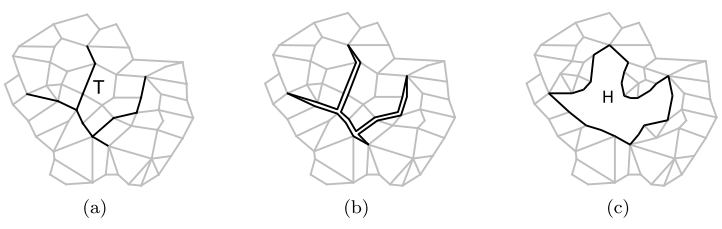
\includegraphics[scale=0.7]{imgs/cut_graph_example.png}
    \caption {Example of cutting process using a subgraph \(T\) to form a face \(H\) inside the graph. (\cite{Borradaile2012}).}
    \label{fig:cut_graph_example}
\end{figure}

% It is worth mentioning that if the subgraph used to do the cutting has cycles, the cutting process may disconnect components of the original graph.

From that, we define a \textbf{cut graph} \(CG\) as a subgraph of \(G\) that when used to cut \(G\) results in a planar graph.

The goal of this section is to find a \textbf{cut graph} \(CG\) of \(G\) that contains all terminals and whose cost is bounded by a constant times \(\opt\). Cutting \(G\) using \(CG\) results in a planar graph with a cycle \(\sigma\) as the boundary, where \(\sigma\) is twice the cost of \(CG\).

Figure~\ref{fig:mortar5} illustrates the process of cutting a graph of genus greater than 0.  Figure~\ref{fig:mortar5}(a) shows a cut graph drawn on a torus, while Figure~\ref{fig:mortar5}(b) shows the result of cutting the surface along the graph: the shaded area is homeomorphic to a disk, and the light area is the additional face of the planarized surface.

\begin{figure}[h]
    \centering
    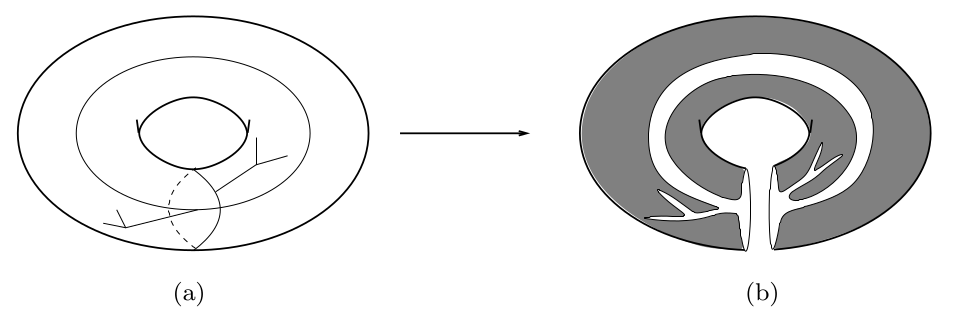
\includegraphics[scale=0.45]{imgs/mortar5.png}
    \caption {Example of a cut in a graph with \textit{genus} greater than zero. (\cite{Borradaile2012}).}
    \label{fig:mortar5}
\end{figure}


\cite{Borradaile2012} observed that, given a planar graph \(G\) and a spanning tree \(T\) of \(G\), the set of edges \(E(G) - E(T)\) induces a spanning tree \(T^{\star}\) in the dual graph \(G^{\star}\). Furthermore, if \(T\) is a minimum spanning tree of \(G\), then \(T^{\star}\) is a maximum spanning tree of \(G^{\star}\). This result was derived by \citeauthor{Borradaile2012} from the Lemma~1 of~\cite{EPPSTEIN199233}.

The result can be generalized for bounded \textit{genus} graphs: if \(T\) is a minimum spanning tree of \(G\) and \(T^{\star}\) is a maximum spanning tree of \(G^{\star} - E(T)\), then \(T^{\star}\) is a maximum spanning tree of \(G^{\star}\) and the size of the set of remaining edges \(X := E(G) - E(T) - E(T^{\star})\) is \(g\), or the Eulerian \textit{genus} of \(G\), obtained by Euler's formula. \cite{Eppstein} define such a triple \((T, T^{\star}, X)\) as the \textit{tree-cotree decomposition} of \(G\), and shows that a cut graph can be generated from this decomposition.

\begin{figure}[H]
    \centering
\begin{tikzpicture}


    \Vertex[x=0, y=2, color=white, Math,IdAsLabel]{A}
    \Vertex[color=white, Math,IdAsLabel]{B}

    \Vertex[x=1, y=1, color=white, Math,IdAsLabel]{C}
    \Vertex[x=2, y=0, color=white, Math,IdAsLabel]{D}

    \Vertex[x=1, y=-0.3, color=white, Math,IdAsLabel]{E}
    \Vertex[x=2, y=1.5, color=white, Math,IdAsLabel]{F}

    \Vertex[x=3, y=0, color=white, Math,IdAsLabel]{G}
    \Vertex[x=3, y=1.5, color=white, Math,IdAsLabel]{H}

    \Edge[opacity=1.0](A)(B)
    \Edge[opacity=0.3](A)(F)
    \Edge[opacity=1.0](A)(C)
    \Edge[opacity=1.0](C)(F)
    
    \Edge[opacity=0.3](A)(E)
    \Edge[opacity=1.0](C)(E)
    \Edge[opacity=0.3](D)(E)


    \Edge[opacity=0.3](F)(H)
    \Edge[opacity=0.3](H)(G)
    \Edge[opacity=0.3](G)(D)
    \Edge[opacity=0.3](D)(F)
    \Edge[opacity=0.3](F)(G)
    \Edge[color=green](D)(H)

    \Edge[color=red](F)(H)
    \Edge[color=red](F)(D)
    

\end{tikzpicture}
    \caption{Example of \(loop(T, e)\). The tree \(T\) is rooted at the vertex \(F\) and is represented by the black (non-opaque) edges. The edge \(e\) is represented in green and the paths between \(e\) and the vertex \(F\) are displayed in red. The \(loop(T, e)\) is composed of the union of the red and green edges.}
    \label{fig:loop_T_e}
\end{figure}


Let \(T\) be a spanning tree rooted at a vertex \(r\), and let \(e\) be an edge not contained in \(T\). We say that \(loop(T, e)\) is the simple cycle formed by \(e\) and the paths between \(r\) and both ends of \(e\) (exemplified in Figure~\ref{fig:loop_T_e}). Based on the results from \citeauthor{Eppstein},~\cite{Borradaile2012} showed in the following result.

\begin{flemma}[\cite{Borradaile2012}, Lemma 1]
    Given a tree-cotree decomposition \((T, T^{\star}, X)\), \(\{loop(T, e): e \in X\}\), induces a cut graph.
\end{flemma}

The construction of the cut graph for our purposes follows from~\cite{Borradaile2012}, with slight technical changes. We start with \(T_i\), which is a minimum spanning tree of the component \(C_i\) calculated in Algorithm~\ref{algorithm:pc-partition}, and contract it to a vertex \(r\).

We then find a shortest-path tree \(SPT\) rooted at \(r\), uncontract \(r\) back into \(T_i\) and set \(T := T_i \cup SPT\), where \(T\) is a spanning tree of \(G\). With that, we can then find a spanning tree \(T^\ast\) of \(G^\ast - E(T)\) using the results presented above.

Let \(X := E(G) - E(T) - E(T^\ast)\). As the output cut graph we return \(CG := T_i \cup \{loop(T, e): e \in X\}\).

We proceed to cut \(G\) using \(CG\) and duplicate each edge and vertex of \(CG\), thus, generating a cycle \(\sigma\) internal to \(CG\). After this process, let \(G_1\) be the planar graph obtained from \(G\). Finally, we invert the face \(\sigma\) in such a way that \(\sigma\) becomes the new external face of \(G_1\). From construction and Theorem~\ref{theoremClustering}, \(c(\sigma)\) is at most \(c \opt\) where \(c\) is a constant.

\citeauthor{Borradaile2012} refers to the algorithm presented above as \textbf{Planarize algorithm} and formalizes the result with the following lemma.

\begin{flemma}[\cite{Borradaile2012}, Lemma 2]
    The algorithm \textbf{Planarize} returns a cut graph \(CG\) such that cutting \(G\) open along \(CG\) results in a planar graph \(G_p\) with face \(f_\sigma\) whose facial walk \(\sigma\)

    \begin{enumerate}
        \item is a simple cycle,
        \item contains all terminals (some terminals might appear more than once as multiple copies might be created during the cutting process); and
        \item has cost \(c(\sigma) \leq c \opt\) for \(c > 0\) constant.
    \end{enumerate}
\end{flemma}

\subsubsection{Strips}

To continue with the algorithm, we need to present the following definition. Given $\epsilon > 0$ and a graph \(G\), a path \(P\) in \(G\) is \(\epsilon\)-\textit{short} if in each pair of vertices \((x, y) \in P\) the distance between \(x\) and \(y\) in \(P\) is at most \((1 + \epsilon)\) times the distance \(x\) and \(y\) in \(G\), in other words, \(dist_P(x, y) \leq (1 + \epsilon) dist_G(x, y)\).

We proceed to decompose the planar graph \(G_1\) into \textit{strips}. Let \(x\) and \(y\) be two vertices in \(\sigma\). Let \(\sigma[x, y]\) be the path between \(x\) and \(y\) in \(\sigma\) in the counterclockwise direction of the \textit{planar embedding} of \(G_1\) into a sphere. If \(x = y\), by convention \(\sigma[x, y] = \sigma\).

In order to segment \(G_1\) into strips, we find vertices \(x\) and \(y\) in \(\sigma\) such that \(\sigma[x, y]\) is the shortest path of \(\sigma\) which is not \(\epsilon\)-\textit{short} in \(\sigma\). Such a pair of vertices always exists since \(\sigma[x, y]\), with \(x = y\), is not \(\epsilon\)-\textit{short}. Let \(N\) be the shortest path between \(x\) and \(y\) in \(G_1\). Certainly \(c(N) < c(\sigma[x, y])\). We call \textbf{strip} the subgraph of \(G_1\) covered by \(N \cup \sigma[x, y]\). This process is performed recursively on the subgraph of \(G_1\) covered by \(N \cup (\sigma - \sigma[x, y])\). As a result, we have \(G_1\) segmented by strips. Items~(a) and (b) of Figure~\ref{fig:mortar2} illustrate this process.

\begin{flemma}[\cite{klein2006}, inequality (10)] \label{strip_length}
The total cost of the boundary of all strips is at most \((\frac{1}{\epsilon} + 1)\) times the cost of \(\sigma\).
\end{flemma}

\citeauthor{klein2006} also showed that the strip decomposition of a planar graph with \(n\) vertices can be found in time \(\mathcal{O}(n \log n)\).

Given a fixed strip, we denote \(N\) as the north-boundary of the strip and \(S\) as the south-boundary.

With the graph \(G_1\) decomposed into strips, as illustrated in Item~(b) of Figure~\ref{fig:mortar2}, the next step is, for each strip, to calculate the shortest paths, called \textit{columns}. Consider a strip with north and south boundaries, \(N\) and \(S\) respectively. We select vertices \(s_0, s_1, \dots\) in \(S\) as follows. We embed the north strip above the south strip, directing \(S\) and \(N\) from left to right. Let \(s_0\) be the leftmost vertex common to \(S\) and \(N\). By convention, the column \(C_0\) is defined as the shortest path between \(s_0\) and \(N\), in this case, an empty path.

For \(i \geq 1\), find the first vertex in \(S\) (from left to right) such that the cost of the path from \(s_{i-1}\) to \(s_i\) in \(S\) is greater than \(\epsilon\) times the cost of the shortest path from \(s_i\) to \(N\) within the strip, that is, \(dist_S(s_{i-1}, s_i) > \epsilon \cdot dist_{strip}(s_i, N)\). Thus, column \(C_i\) is defined as the shortest path between \(s_i\) and \(N\) in the strip, as illustrated by Item~(c) of Figure~\ref{fig:mortar2}.

\begin{figure}[H]
    \centering
    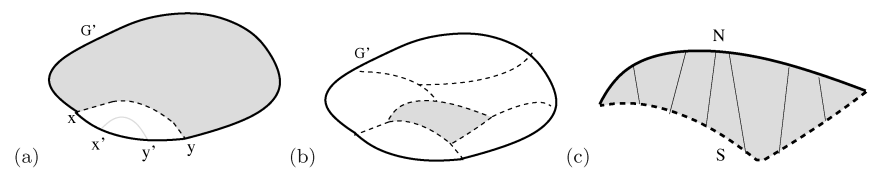
\includegraphics[scale=0.5]{imgs/mortar2.png}
    \caption{Construction of strips in Mortar Graph (\cite{Borradaile2009b}).}
    \label{fig:mortar2}
\end{figure}

In Figure~\ref{fig:mortar2}, Item~(a) shows the first track is created by a path (dashed) connecting \(x\) and \(y\). The distance between every pair of vertices \(x'\) and \(y'\), between \(x\) and \(y\) on the boundary, is well approximated by the distance on the boundary. We use recursion in the shaded area; Item~(b) shows how a graph is divided into bands (by the dashed lines). A strip is increased in Item~(c). Columns (vertical lines) are taken from the set of shortest paths between the ``low'', or south boundary (dashed line) and the ``up'', or north boundary (solid line).

\begin{flemma}[\cite{klein2006}, Lemma 5.2]
The sum of all column costs in a strip is at most \(\epsilon^{-1} \cdot c(S)\).
\end{flemma}

After having the columns calculated, for each strip, we have a set \(C_0, C_1, \dots, C_s\) of columns of the strip.

For \(\epsilon > 0\), let \(\kappa = \kappa(\epsilon) = 4 \epsilon ^ {-2} (1 + \epsilon ^ {-1})\). We will use this constant on the following definition and for the following lemmas due to \cite{Borradaile2009b}.

% Let \(\mathcal{C}_i = C_i \cup C_{i+\kappa} \cup C_{i+2\kappa} \cup \dots\) for \(i \in \{0, 1, \dots, \kappa - 1\}\).
Let \(\mathcal{C}_i = \bigcup_{j=0}^{\kappa-1} C_{i+j\kappa}\) for \(i \in \{0, 1, \dots, \kappa - 1\}\).

Let \(i^\ast\) be the index that minimizes \(c(\mathcal{C}_i)\). We designate the columns of \(\mathcal{C}_i^\ast\) as \textbf{super-columns}.

\begin{flemma}[\cite{Borradaile2009b}, Lemma 6.5]
The sum of the costs of the super-columns in a strip is at most \(\kappa^{-1}\) times the sum of the costs of the columns in the strip.
\end{flemma}

\begin{flemma}[\cite{Borradaile2009b}, Lemma 6.6] \label{borradaile_2009b_lemma_6_6}
     The sum of the costs of all the super-columns over all strips is at most \(c \epsilon \opt\), where \(\epsilon > 0\) and \(c > 0\) depends on \(\epsilon\).
\end{flemma}

We define as the \textbf{Mortar Graph} \(MG\) of \(G\) the embedded planar subgraph generated by the edges of \(T_i\), the edges of the strips, and the edges of super-columns. This is illustrated in Item~(b) of Figure~\ref{fig:mortar3}.

We note two properties derived from the results presented during the construction of \(MG\). First, let \(Q\) be the set of all terminals of \(G\), by construction, we have that \(Q \subseteq V(MG)\). The second property is presented below.

\begin{flemma} \label{length_mg}
     \(c(MG) \leq k \epsilon c(\sigma)\) with \(k > 0\) constant.
\end{flemma}
\begin{proof}
    The result follows from Theorem~\ref{theoremClustering} and Lemmas~\ref{strip_length} and~\ref{borradaile_2009b_lemma_6_6}.
\end{proof}

\subsubsection{Bricks}

To create a \textbf{brick} (illustrated in  Figure~\ref{fig:mortar3}(c)), for each face \(f\) of \(MG\), we duplicate the border edges and vertices of \(f\). This results in a disconnected induced subgraph of \(G_1\) that is entirely contained within the ``external'' copy of \(f\)'s border (Figure~\ref{fig:mortar4}(c)). The result of this process can be seen in Figure~\ref{fig:mortar4}.

Figure~\ref{fig:mortar4}(a) illustrates the boundary of a face \(f\) of \(MG\) as a cycle of edges (thick edges), possibly with repetition (that is, an edge can occur twice at the border). The light edges are those inside \(f\) in \(G\). Figure~\ref{fig:mortar4}(b) shows an example of brick \(B\) obtained by the process described above. \(B\) has boundary \(\partial B\). Figure~\ref{fig:mortar4}(c) shows a brick \(B\) contained within the ``external'' copy of the border of \(f\).

\begin{figure}[h]
    \centering
    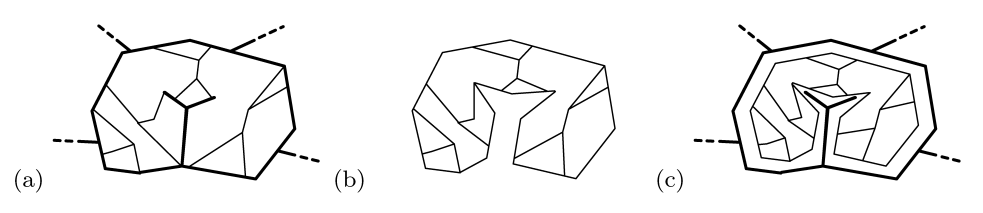
\includegraphics[scale=0.45]{imgs/mortar4.png}
    \caption{Construction of a brick. (\cite{Borradaile2009b}).}
    \label{fig:mortar4}
\end{figure}

The boundary \(\partial B\) of a brick \(B\) is the simple cycle formed by the edges of the boundary. The corresponding face of \(MG\) is called \textbf{mortar boundary} from~\(B\). Each edge of \(MG\) occurs at most in the disjoint union of the boundary of the bricks.

\begin{flemma}[\cite{Borradaile2009b}, Lemma 6.10]
    A mortar boundary \(B\), in counterclockwise order, is the concatenation of four paths \(W\), \(S\), \(E\), \(N\) (west, south, east, north) such that:
    \begin{enumerate}
        \item The set of edges \(B - \partial B\) is nonempty.
        \item Every vertex of \(\mathcal{D} \cap B\) is in \(N\) or in \(S\).
        \item \(N\) is \(0\)-short in \(B\), and every proper subpath of \(S\) is \(\epsilon\)-short in S.
        \item There exist \(k \leq \kappa\) vertices \(s_0, s_1, s_2, \dots, s_k\) ordered from west to east along \(S\) such that, for any vertex \(x\) of \(S[s_i, s_{i+1})\), the distance from \(x\) to \(s_i\) along \(S\) is less than \(\epsilon\) times the distance from \(x\) to \(N\) in \(B\), that is, \(dist_S(x, s_i) < \epsilon dist_B(x, N)\).
    \end{enumerate}
\end{flemma}

\subsubsection{Portals}

The connection between a face \(f\) of \(MG\) and its respective brick \(B\) is performed through a subset of vertices of \(\partial B\) called \textbf{portals}. This connection is made in such a way that, for each portal \(p\) of \(\partial B\), an edge with weight 0 is placed between \(p\) and the vertex of which it was duplicated in \(\partial f\).

For each brick \(B\), we set some vertices of \(\partial B\) as \textbf{portals}. We define \(\theta = \theta(\epsilon) = 18 \cdot \alpha(\epsilon) \cdot \epsilon ^ {-2}\). Where \(\alpha(\epsilon)\) is a constant that will be defined later.

For portal selection, we use the following greedy algorithm. An initial vertex \(v_0\) of \(\partial B\) is selected with uniform probability. Then we define \(v_1\) as the first vertex of \(\partial B\) clockwise such that \(c(\partial B[v_0, v_1]) > c(\partial B) / \theta\). This process is repeated for \(v_i\) in \(\partial B\) until \(v_0 \in V(\partial B (v_{i-1}, v_i))\).

Using the previous construction, we get the following properties given by \cite{Borradaile2009b}.

\begin{flemma}[\cite{Borradaile2009b}, Lemma 7.1] \label{lemma:cobertura}
(Cover property): For any vertex \(x \in \partial B\), there exists a portal \(y\) such that the \(x\)-to-\(y\)-subpath of \(\partial B\) has a maximum cost \(c(\partial B) / \theta\).
\end{flemma}

\begin{flemma}[\cite{Borradaile2009b}, Lemma 7.2]
(Cardinality property): There are at most \(\theta\) portals in \(\partial B\).
\end{flemma}

With that, we have a Mortar Graph \(MG\) with a set of bricks connected with the face boundaries of \(MG\) through portal edges, as illustrated by Item~(d) Figure~\ref{fig:mortar3}. This construction is named by \citeauthor{Borradaile2009b} as \textbf{portal-connected graph}, and is denoted as \(\mathcal{B}^{+}(MG)\).

\begin{figure}[H]
    \centering
    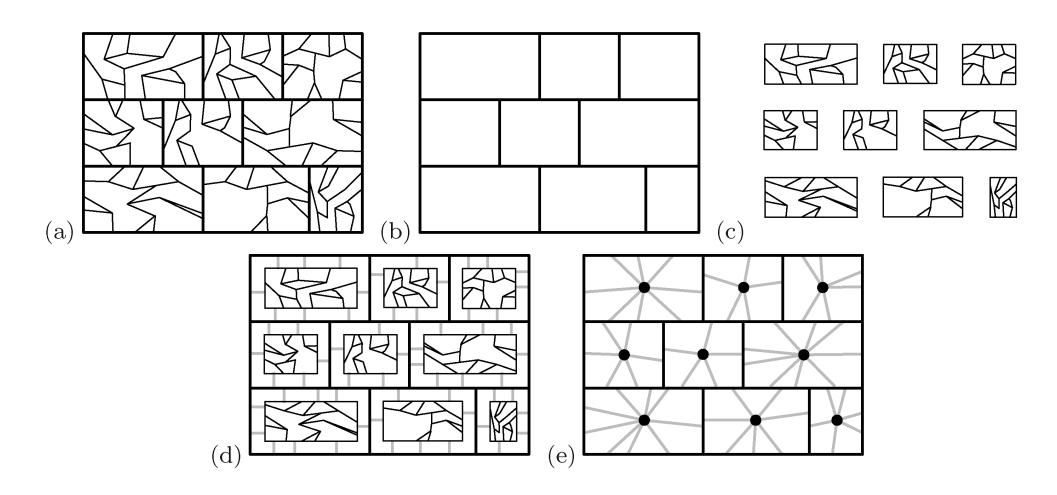
\includegraphics[scale=0.4]{imgs/mortar3.png}
    \caption{Mortar Graph. (\cite{Borradaile2009b}).}
    \label{fig:mortar3}
\end{figure}

Figure~\ref{fig:mortar3} shows in Item~(a) the graph \(G_1\), highlighting the edges of the Mortar Graph. 
Item~(b) shows only the Mortar Graph \(MG\) obtained. 
Item~(c) shows the set of bricks corresponding to \(MG\) (those will be defined ahead). 
Item~(d) illustrates a portal-connected graph \(\mathcal{B}^{+}(MG)\) (will be presented ahead), where the portal edges are gray. 
Item~(e) shows \(\mathcal{\mathcal{B}}^{+}(MG)\) with the bricks contracted into vertices, resulting in \(\mathcal{B}^{\div}(\mathcal{B }^{+}(MG))\).

\subsection{Spanner construction}

Finally, we proceed to prove Theorem~\ref{theorem:spanner}.

We start by building a separate subgraph \(H_i\) for each \(T_i\). Let \(H_i\) be a Mortar Graph created from \(T_i\). Following that, for each brick \(B\) and a selection of its portals \(\Pi' \subseteq \Pi\), we add to \(H_i\) an optimal Steiner Tree that reaches \(\Pi'\) and uses only edges from the interior of \(B\) or its boundary. This can be done in polynomial time in \(\theta\) using the algorithm proposed in \cite{ericksonST}, since all terminals lie on the infinite face of a planar graph.

Note that for fixed \(\epsilon\) and \(g\) there is at most a constant number of portals, hence a constant number of such Steiner Trees, and the cost of each is at most the cost of the boundary of the brick \(B\).

We will leverage an auxiliary result to prove both spanner properties.

\begin{flemma}\label{lemma:borradaile_10_1}
    Let \(G\) be a planar embedded graph and let \(C\) be a subgraph of \(G\) that intersects a \(\epsilon\)-short path \(P\). There is a subpath of \(P\) spanning the vertices of \(C \cap P\) whose total cost is \((1 + \epsilon) c(C)\)
\end{flemma}
\begin{proof}
    Let \(P'\) be the shortest subpath of \(P\) that spans all the vertices of \(C \cap P\). There is a path \(Q\) in \(C\) that connects all vertices of \(C \cap P\). Since \(P\) is \(\epsilon\)-short \(c(P') \leq (1 + \epsilon)c(Q) \leq (1 + \epsilon)c(C)\).
\end{proof}

\begin{flemma} [\cite{Bateni}, Lemma 4.1] \label{bateni_4_1_forest}
    For any forest \(F\) in a brick \(B\), there exists a forest \(F'\) such that
\begin{enumerate}
    \item \(c(F') \leq (1 + \epsilon)c(F)\);
    \item \(F'\) crosses the boundary of \(B\) at most \(\alpha\) times; and
    \item any two vertices on \(N\)- or \(S\)-boundaries of \(B\) connected by \(F\) are also connected by \(F'\)
\end{enumerate}
\end{flemma}

In Corollary~\ref{bateni_4_1_multicycle}, we will generalize the result above to a collection of cycles (instead of a forest), but first, we need to introduce the concept of \textbf{cleaving}.

Put simply, cleaving is the process of breaking a vertex into two new vertices and adding an artificial, zero-cost edge between them. It can be formalized as: given a vertex \(v\) and a bipartition \(A, B\) of the edges incident to \(v\), split \(v\) into two new vertices \(v_A\) and \(v_B\). Then, connect the endpoints of the edges in \(A\), previously connected to \(v\), to \(v_A\), and the edges in \(B\) to \(v_B\). Finally, add a zero-cost edge \(e_{AB}\) between \(v_A\) and \(v_B\). This operation is illustrated in Figure~\ref{fig:cleaving} (a) and (b).

There can be two types of cleaving:
\begin{itemize}
    \item Simplifying Cleaving (Figure~\ref{fig:cleaving} (c) and (d)). Let \(C\) be a clockwise, non-self-crossing (i.e., planar) non-simple cycle that visits a vertex \(v\) twice. Defined a bipartition of the edges incident to \(v\) as follows: given the clockwise embedding of the edges incident to \(v\), let \(A\) start and end with consecutive edges of \(C\) and contain only two edges of \(C\), let \(B\) be the remaining edges. Such a bipartition exists because \(C\) is non-self-crossing.
    \item Lengthening Cleaving (Figure~\ref{fig:cleaving} (e) and (f)). Let \(C\) be a simple cycle, and let \(v\) be a vertex on \(C\) with two edges \(e_A\) and \(e_B\) adjacent to \(v\) embedded strictly inside \(C\), and let \(e'_A\) and \(e'_B\) be consecutive edges of \(C\) adjacent to \(v\) such that the following bipartition is non-crossing concerning the embedding: \(A\), \(B\) is a bipartition of the edges adjacent to \(v\) such that \(e_A, e'_A \in A\) and \(e_B, e'_B \in B\).
\end{itemize}

\begin{figure}[h]
    \centering
    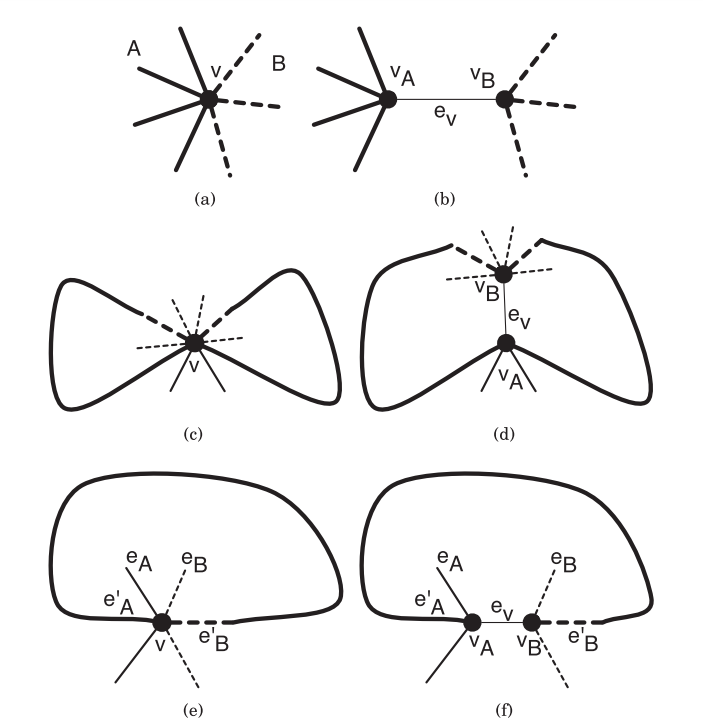
\includegraphics[scale=0.5]{imgs/cleaving.png}
    \caption{Cleavings illustrated (\cite{borradaile_2EC}).}
    \label{fig:cleaving}
\end{figure}

\begin{fcorollary}\label{bateni_4_1_multicycle}
For any collection of cycles \(M\) in a brick \(B\), there is a collection of cycles \(M'\) such that
\begin{enumerate}
    \item \(c(M') \leq (1 + c \epsilon)c(M)\)
    \item \(M'\) crosses the boundary of \(B\) at most an \(\alpha\) (constant) number of times
    \item any two vertices on \(N\)- or \(S\)-boundaries of \(B\) connected by \(M\) are also connected by \(M'\)
\end{enumerate}
\end{fcorollary}
\begin{proof}
    Let \(M^\ast\) be an optimal solution to the SMCP in \(G\) and let \(MG\) be a Mortar Graph built from \(G\). 

    For a given brick \(B\) (with \(W, N, E, S\) boundaries), let \(M\) be the intersection between \(M^\ast\) and \(B\). Note that \(M\) might be composed of cycles and trees (e.g., cycle fragments that connect to themselves outside the brick) and each vertex in \(M \cap \partial B\).

    We begin the construction of \(M_1\) by adding the \(W\) and \(E\) boundaries of \(B\) to \(M\). We know from Lemma~\ref{borradaile_2009b_lemma_6_6} that the cost of the union of \(M^\ast\) with all super-columns (i.e., the west and east boundaries of all bricks) is at most \((1 + 2 c \epsilon) \opt\).

    To streamline the rest of the proof, we perform the simplifying cleaving on non-simple cycles of \(M_1\) until all cycles become simple (also accounting for duplicated edges).
    We can have two situations for each component \(C\) of \(M_1\):
    \begin{enumerate}
        \item \(C\) connects vertices in \(N\) or vertices in \(S\)
        \item \(C\) connects vertices from \(N\) and \(S\)
    \end{enumerate}

    To tackle case (1), we use Lemma~\ref{lemma:borradaile_10_1} to replace the path of \(C\) that connects two vertices in \(N\) with a subpath of \(N\), which connects the same vertices. Since \(N\) is a \(\epsilon\)-path, the Lemma holds, and the increase in cost is limited by a \((1 + \epsilon)\) factor.

    For case (2), we apply the lengthening cleaving to the boundary of brick \(B\). For each vertex \(v\) in \(M_1 \cap \partial B\) that has a degree greater than one, we perform the lengthening cleaving in \(v\). We repeat this process while there are still multiple edges of the solution embedded in a brick that is incident to a shared boundary vertex. In other words, we have that the intersection of \(M_1\) with the interior of brick \(B\) is a subgraph whose joining vertices with \(\partial B\) have degree one.


    The first property follows, since - as mentioned - in case (1), the increase in cost is limited by a \((1 + \epsilon)\) factor, and in case (2) we only add zero-cost edges.
    
    To get the second and third properties, we can directly apply Lemma~\ref{bateni_4_1_forest} (Structural properties of Bricks) on \(M_1\). 
\end{proof}

Considering the final spanner \(H\) to be the union of all \(H_i\)'s, we proceed to prove that \(H\) indeed respects both properties of \textbf{quasi-optimality} and \textbf{shortness}.

\begin{flemma}{{(Shortness property).}}\label{spanner_shortness_property} Given a graph \(G\) and a subgraph \(H\) of \(G\) constructed with the process above, the cost of \(H\) is at most \(f(\epsilon, g) \opt\) for a certain function
\(f(\epsilon, g)\).
\end{flemma}
\begin{proof}
Note that each \(H_i\) is constructed from \(MG_i\) (which by its turn is built from \(T_i\)), a set of portal edges connected to \(MG_i\), and a limited set of Steiner Trees inside the bricks. By Lemma~\ref{length_mg}, \(c(MG_i) \leq f(\epsilon, g) c(T_i)\). For each brick \(B\), we add at most \(2^{\theta}\) trees, each with cost no more than \(c(\partial B)\). Since each edge of \(MG_i\) may appear in at most two bricks, the total cost is bounded by \(2^{\theta + 1} c(MG_i)\). Therefore, \(c(H_i) \leq 2^{\theta + 1} c(MG_i) = f(\epsilon, g) c(T_i)\).

By Theorem~\ref{theoremClustering}, the sum of the cost of all \(T_i\) is no more than \((16/\epsilon + 4) \opt_{\mathcal{D}}(G_{in})\).
This implies that the sum of the cost of all \(H_i\) is no more than \(f(\epsilon, g) (16/\epsilon + 4) \opt_{\mathcal{D}}(G_{in})\).
\end{proof}

\begin{flemma}\label{spanner_quasi_optimality_property}
    Quasi-optimality property.~\(\opt_{\mathcal{D}}(H) \leq (1 + c \epsilon) \opt_{\mathcal{D}}(G_{in})\) with \(c\) and \(\epsilon\) constants.
\end{flemma}
\begin{proof}

    Let \(\{C_i\}_{i=1}^k\) be the set of components outputted by Algorithm~\ref{algorithm:pc-partition}.

    From Theorem~\ref{theoremClustering}, we have that \(\sum_{i}^k \opt_{\mathcal{D}_i} \leq (1 + \epsilon) \opt_{\mathcal{D}}\). So we can focus on proving that \(\opt_{\mathcal{D}_i}(H_i) \leq (1 + c \epsilon) \opt_{\mathcal{D}_i}(G_{in})\).

    Consider each \(H_i\) as formed in the process above, so each \(H_i\) is formed by a Mortar Graph built using \(T_i\) (a minimum spanning tree of \(C_i\) from Theorem~\ref{theoremClustering}), the portal edges and the set of Steiner Trees connecting the portals in each Brick.

    Let \(M^\ast_i\) be an optimal solution for the SMCP considering \(\mathcal{D}_i\), i.e. \(c(M^\ast_i) = \opt_{\mathcal{D}_i}(G_{in})\). We add the set of all super-columns in \(H_i\) to \(M^\ast_i\) to get \(M^1_i\). Recall that, by Lemma~\ref{borradaile_2009b_lemma_6_6}, the cost of these super-columns is at most \(c \epsilon \opt_{\mathcal{D}_i}(G_{in})\).

    Next, we replace the intersection of \(M_i^1\) and each brick with another subgraph having the properties of  Corollary~\ref{bateni_4_1_multicycle}. Let \(M_i^2\) be the new subgraph. The cost of the solution increases to no more than a \(1 + c \epsilon\) factor.

    From  Corollary~\ref{bateni_4_1_multicycle}, we know that \(M_i^2\) crosses each brick at most \(\alpha\) times, so we can ensure that moving these intersection points to the portals adds no more than a constant factor in the cost.

    Consider a brick \(B\) with boundaries \(W, N, E, S\). Connect each intersection point of the brick to its closest portal. Each connection on a brick \(B\) moves by at most \(2 c(\partial B) / \theta\). Therefore, the total movement of each brick is at most \(\alpha 2 c(\partial B) / \theta\), which is no more than \(2 \epsilon^2 c(\partial B) / \gamma(\epsilon, g)\). Hence, the total additional cost for all bricks of \(H_i\) is bounded by \(4 \epsilon^2 c(T_i)\). Let \(M_i^3\) be the resulting subgraph.

    Hence the cost of \(M_i^3\) is at most \(4 \epsilon^2 c(T_i) + c(M_i^2)\). Considering that \(c(M_i^2) \leq (1 + \epsilon) c(M_i^1)\) and \(c(M_i^1) \leq \epsilon^2 c(T_i) + M^\ast_i\), we have that \(c(M_i^3) \leq 4 \epsilon^2 c(T_i) + (1 + \epsilon) c(M^\ast_i)  + \epsilon^2 c(T_i)\)

    Let \(M' = \bigcup_i^k M_i^3\). Accounting that \(\sum_i^k c(T_i) \leq (4/\epsilon + 4) \opt\) (from Theorem~\ref{theoremClustering}), it holds that \[c(M') \leq \sum_i^k \left ( 4 \epsilon^2 c(T_i) + (1 + \epsilon) c(M^\ast_i)  + \epsilon^2 c(T_i) \right).\] 
    Therefore, we can conclude that  \(c(M') \leq (1 + 21 \epsilon + 20 \epsilon^2) \opt = (1 + c'\epsilon) \opt\).
\end{proof}


\section{PTAS for Graphs of Bounded Genus}
\label{section:ptas_bounded_genus}

We can now prove one of the main results of this work, which is a PTAS for the Steiner Multicycle Problem on graphs with bounded genus.

First, we state an auxiliary result from \cite{Demaine2010}.

\begin{ftheo}[\cite{Demaine2010} Theorem 1.1] \label{demaineResult}
    For a fixed genus \(g\), and any integer \(k \geq 2\) and for every graph \(G\) of Euler genus at most \(g\), the edges of \(G\) can be partitioned into \(k\) sets such that contracting the edges in any of the sets results in a graph of treewidth \(\mathcal{O}((g + 1)^2k)\). Furthermore, such a partition can be found in \(\mathcal{O}((g+ 1)^{5/2} n^{3/2} \log{n})\) time.
\end{ftheo}

The proposed PTAS algorithm is presented in Algorithm~\ref{smcp-ptas}.

\begin{algorithm}
\caption{SMCP-PTAS}
\label{smcp-ptas}
\begin{algorithmic}[1]

\Require Graph \(G_{in}\) of bounded genus \(g\), a set of terminal pairs \(\mathcal{D}\), and a constant \(1 \geq \epsilon > 0\).
\Ensure A collection of cycles satisfying \(\mathcal{D}\) whose cost is at most \((1 + c' \epsilon) \opt\)
\State  \(\epsilon' \gets \epsilon / 6\)
\State  \(k \gets \max\left \{ f(g, \epsilon')/{\epsilon'}, \: 2\right \}\); \(f(g, \epsilon')\) as in Lemma~\ref{spanner_shortness_property} \label{alg_smcp_ptas:k}
\State Construct a spanner \(H\) of \(G_{in}\) \label{alg_smcp_ptas:SpannerCall}
\State Use Theorem~\ref{demaineResult} to partition the edges of \(H\) into \(E_1, \dots, E_k\) \label{alg_smcp_ptas:partDemaine}
\State  \(j^\ast \gets \arg\min\limits_{j \in \{1,\ldots,k\}} c(E_j)\)
\State Find a \((1 + k \epsilon)\) collection of cycles (multiset of edges) \(M^\ast\) with respect to \(\mathcal{D}_i\) in \(H/E_{j^\ast}\) using Theorem~\ref{dynamicProgramming}, and with \(k\) constant \label{alg_smcp_ptas:dp}
\State \(M \gets M^\ast \cup E_{j^\ast}\)
\State \Return  \(M\)

\end{algorithmic}
\end{algorithm}

\begin{ftheo}
    The collection of cycles \(M\) produced by Algorithm~\ref{smcp-ptas} on input $(G_{in}, \mathcal{D})$ is a feasible solution for the SMCP and has cost at most \((1 + c' \epsilon) \opt\), with \(c'\) and \(\epsilon\) constants.
\end{ftheo}
\begin{proof}

    In the line~\ref{alg_smcp_ptas:SpannerCall} of Algorithm~\ref{smcp-ptas}, we construct a spanner \(H\) of \(G_{in}\), which respects the properties described in Lemma~\ref{spanner_quasi_optimality_property} and Lemma~\ref{spanner_shortness_property}, that is:

    \begin{itemize}
        \item \(c(H) \leq f(g, \epsilon) \opt\), with \(f(g, \epsilon)\) being a constant that depends on \(\epsilon\) and the genus \(g\) of \(G_{in}\);
        \item \(\opt_{\mathcal{D}}(H) \leq (1 + c \epsilon) \opt_{\mathcal{D}} (G_{in})\).
    \end{itemize}

    Note that Lemma~\ref{spanner_quasi_optimality_property} implies that there is a feasible solution for the SMCP contained in \(H\).

    In line~\ref{alg_smcp_ptas:partDemaine}, we proceed to partition \(H\) using Theorem~\ref{demaineResult}. We choose \(k\) such that \(k = \max( \frac{f(g, \epsilon)}{\epsilon}, 2)\) where \(f(g, \epsilon)\) is the constant from Lemma~\ref{spanner_shortness_property}. 
    
    From Lemma~\ref{demaineResult}, by splitting \(H\) into \(k\) edges sets, we have \(c(E_{j^\ast}) \leq \epsilon \opt\). Moreover, contracting \(E_{j^\ast}\) from \(H\) produces a graph of treewidth \(\mathcal{O}((g +1)^2 k)\).

    Before contracting \(H\) with \(E_{j^\ast}\), we need to do a small treatment of the terminals contained in \(E_{j^\ast}\). We create a new vertex for each terminal in \(E_{j^\ast}\) and connect it to the terminal with a new edge of cost zero. This new vertex will serve as a ``temporary'' terminal in \(H / E_{j^\ast}\). Note that this process does not increase the cost of the final solution, as all added edges have cost zero.

    In line~\ref{alg_smcp_ptas:dp} of Algorithm~\ref{smcp-ptas}, we can find a solution \(M^\ast\) in \(H / E_{j^\ast}\) via Theorem~\ref{dynamicProgramming} and Theorem~\ref{demaineResult}. The cost of \(M^\ast\) is at most \((1 + 2 \kappa \epsilon) \opt\), with \(\kappa = \kappa(\epsilon) = 4 \epsilon ^ {-2} (1 + \epsilon ^ {-1})\).

    Finally, we join the solution \(M^\ast\) with the edges in \(E_{j^\ast}\). To guarantee the feasibility of the union as a solution, we duplicate each edge in \(E_{j^\ast}\). Note that the cost of \(E_{j^\ast}\) accounting for the duplication is at most \(2 \frac{c(H)}{k}\), which equals \(2 \frac{f(g, \epsilon) c(G_{in})}{f(g, \epsilon) / \epsilon} = 2 \epsilon \cdot c(G_{in})\).

    From Theorem~\ref{dynamicProgramming}, we have that \(c(M^\ast) \leq (1 + 2 \kappa \epsilon \opt)\). So \(c(M^\ast \cup E_{j^\ast}) \leq (1 + (2 \kappa + 2) \epsilon) \opt\) holds, and by considering a constant \(c' = 2 \kappa + 2\), we have \(c(M) \leq (1 + c' \epsilon) \opt\).

\end{proof}

The running time of the algorithm, excluding the bounded treewidth PTAS, is bounded by \(\mathcal{O}(n^2 \log n)\). Moreover, the running time of the current procedure for solving bounded treewidth instances is bounded by a polynomial, where \(k\) and \(\epsilon\) appear in the exponent.
